\documentclass{article}

%----
%  Colin Tan
%  Basic setup for homework
%----
%----------------------------------------------------------------------------------------
%	PACKAGES AND OTHER DOCUMENT CONFIGURATIONS
%----------------------------------------------------------------------------------------

\usepackage{fancyhdr} % Required for custom headers
\usepackage{lastpage} % Required to determine the last page for the footer
\usepackage{extramarks} % Required for headers and footers
\usepackage{graphicx} % Required to insert images

\usepackage{listings} % listing codes

\usepackage{siunitx} % SI units
\usepackage{amsmath, amssymb} % Math

\usepackage{tikz} % Drawing graphs
\usepackage{pgfplots} % Drawing mathematical plots
\usepgfplotslibrary{fillbetween}
\pgfplotsset{compat=1.10} % pgf compatable version
\usepackage{float} % Flotation control

\usepackage{framed} % Framing answers
\usepackage{enumitem} % Customize enumeration style

\usepackage{multicol} % Required for columizing
\usepackage{caption} % For non-numbered captions
\usepackage{subcaption} % for caption of subfigures

\usepackage[us]{datetime} % Print date in US format

% Margins
\topmargin=-0.45in
\evensidemargin=0in
\oddsidemargin=0in
\textwidth=6.5in
\textheight=9.0in
\headsep=0.25in 

\linespread{1.1} % Line spacing

% Set up the header and footer
\pagestyle{fancy}
\lhead{\hmwkAuthorName} % Top left header
\chead{\hmwkClass\ (\hmwkClassInstructor\ \hmwkClassTime): \hmwkTitle} % Top center header
\rhead{\firstxmark} % Top right header
\lfoot{\lastxmark} % Bottom left footer
\cfoot{} % Bottom center footer
\rfoot{Page\ \thepage\ of\ \pageref{LastPage}} % Bottom right footer
\renewcommand\headrulewidth{0.4pt} % Size of the header rule
\renewcommand\footrulewidth{0.4pt} % Size of the footer rule

\setlength\parindent{0pt} % Removes all indentation from paragraphs

%----------------------------------------------------------------------------------------
%	DOCUMENT STRUCTURE COMMANDS
%----------------------------------------------------------------------------------------

% Header and footer for when a page split occurs within a problem environment
\newcommand{\enterProblemHeader}[1]{
	\nobreak\extramarks{#1}{#1 continued on next page\ldots}\nobreak
	\nobreak\extramarks{#1 (continued)}{#1 continued on next page\ldots}\nobreak
}

% Header and footer for when a page split occurs between problem environments
\newcommand{\exitProblemHeader}[1]{
	\nobreak\extramarks{#1 (continued)}{#1 continued on next page\ldots}\nobreak
	\nobreak\extramarks{#1}{}\nobreak
}

\setcounter{secnumdepth}{0} % Removes default section numbers
\newcounter{homeworkProblemCounter} % Creates a counter to keep track of the number of problems

\newcommand{\homeworkProblemName}{}
\newenvironment{homeworkProblem}[1][Problem \arabic{homeworkProblemCounter}]{ % Makes a new environment called homeworkProblem which takes 1 argument (custom name) but the default is "Problem #"
	\stepcounter{homeworkProblemCounter} % Increase counter for number of problems
	\renewcommand{\homeworkProblemName}{#1} % Assign \homeworkProblemName the name of the problem
	\section{\homeworkProblemName} % Make a section in the document with the custom problem count
	\enterProblemHeader{\homeworkProblemName} % Header and footer within the environment
}{
	\exitProblemHeader{\homeworkProblemName} % Header and footer after the environment
}

\newcommand{\problemAnswer}[1]{ % Defines the problem answer command with the content as the only argument
	\noindent\begin{oframed}
		#1
	\end{oframed}
}

\newcommand{\homeworkSectionName}{}
\newenvironment{homeworkSection}[1]{ % New environment for sections within homework problems, takes 1 argument - the name of the section
	\renewcommand{\homeworkSectionName}{#1} % Assign \homeworkSectionName to the name of the section from the environment argument
	\subsection{\homeworkSectionName} % Make a subsection with the custom name of the subsection
	\enterProblemHeader{\homeworkProblemName\ [\homeworkSectionName]} % Header and footer within the environment
}{
	\enterProblemHeader{\homeworkProblemName} % Header and footer after the environment
}

%----------------------------------------------------------------------------------------
%	TITLE PAGE
%----------------------------------------------------------------------------------------

\title{
\vspace{2in}
\textmd{\textbf{\hmwkClass:\ \hmwkTitle}}\\
\normalsize\vspace{0.1in}\small{Due\ on\ \hmwkDueDate}\\
\vspace{0.1in}\large{\textit{\hmwkClassInstructor\ \hmwkClassTime}}
\vspace{3in}
}

\author{\textbf{\hmwkAuthorName}}
\date{\today} % Insert date here if you want it to appear below your name

\usetikzlibrary{shapes.geometric, calc}
%\everymath{\displaystyle}
%----------------------------------------------------------------------------------------
%	NAME AND CLASS SECTION
%----------------------------------------------------------------------------------------

\newdate{DueDate}{04}{02}{2015} % Due date in {dd}{mm}{yyyy}
\newcommand{\hmwkTitle}{Homework\ 3} % Assignment title
\newcommand{\hmwkDueDate}{\dayofweekname{\getdateday{DueDate}}{\getdatemonth{DueDate}}{\getdateyear{DueDate}} \displaydate{DueDate}} % Due date
\newcommand{\hmwkClass}{PHYS\ 161} % Course/class
\newcommand{\hmwkClassTime}{11:00am} % Class/lecture time
\newcommand{\hmwkClassInstructor}{Professor Landee} % Teacher/lecturer
\newcommand{\hmwkAuthorName}{Zhuoming Tan} % Your name

%----------------------------------------------------------------------------------------

\begin{document}

\maketitle
\newpage
%----------------------------------------------------------------------------------------
%	TABLE OF CONTENTS
%----------------------------------------------------------------------------------------

%\setcounter{tocdepth}{1} % Uncomment this line if you don't want subsections listed in the ToC

%\newpage
%\tableofcontents
%\newpage

%----------------------------------------------------------------------------------------
%	PROBLEM 1
%----------------------------------------------------------------------------------------

% To have just one problem per page, simply put a \clearpage after each problem

\begin{homeworkProblem}
	(II-20) In cylindrical coordinates... (problem omitted)
	% Question

	\problemAnswer{
		For the top and bottom surfaces,
		\[
			\iint_{S_3}\mathbf{F}\cdot\hat{\mathbf{n}}\,dS=\iint_{S_3}F_z\,dS\simeq F_z\left(r,\theta,z+\frac{\Delta z}{2}\right)r\Delta r\Delta\theta
		\]
		\[
			\iint_{S_4}\mathbf{F}\cdot\hat{\mathbf{n}}\,dS=-\iint_{S_4}F_z\,dS\simeq-F_z\left(r,\theta,z-\frac{\Delta z}{2}\right)r\Delta r\Delta\theta
		\]
		so
		\[
			\frac{1}{\Delta V}\iint_{S_3+S_4}\mathbf{F}\cdot\hat{\mathbf{n}}\,dS\simeq\frac{1}{\Delta z}\left[F_z\left(r,\theta,z+\frac{\Delta z}{2}\right)-F_z\left(r,\theta,z-\frac{\Delta z}{2}\right)\right]
		\]
		So as $\Delta z\rightarrow0$, this becomes $\frac{\partial F_z}{\partial z}$. For the side surfaces,
		\[
			\iint_{S_5}\mathbf{F}\cdot\hat{\mathbf{n}}\,dS=\iint_{S_5}F_\theta\,dS\simeq F_\theta\left(r,\theta+\frac{\Delta\theta}{2},z\right)\Delta r\Delta z
		\]
		\[
			\iint_{S_6}\mathbf{F}\cdot\hat{\mathbf{n}}\,dS=-\iint_{S_6}F_\theta\,dS\simeq-F_\theta\left(r,\theta-\frac{\Delta\theta}{2},z\right)\Delta r\Delta z
		\]
		so
		\[
			\frac{1}{\Delta V}\iint_{S_5+S_6}\mathbf{F}\cdot\hat{\mathbf{n}}\,dS\simeq\frac{1}{r\Delta\theta}\left[F_\theta\left(r,\theta+\frac{\Delta\theta}{2},z\right)-F_\theta\left(r,\theta-\frac{\Delta\theta}{2},z\right)\right]
		\]
		So as $\Delta\theta\rightarrow0$, this becomes $\frac{1}{r}\frac{\partial F_\theta}{\partial\theta}$.
	}
\end{homeworkProblem}

%----------------------------------------------------------------------------------------
%	PROBLEM 2
%----------------------------------------------------------------------------------------

\begin{homeworkProblem}
	(II-21) Repeat Problem II-20 to... (problem omitted)
	% Question

	\problemAnswer{
		In spherical coordinates, $\Delta V=r^2\sin\phi\Delta r\Delta\phi\Delta\theta$. For the surfaces in $r$ direction,
		\[
			\iint_{S_1}\mathbf{F}\cdot\hat{\mathbf{n}}\,dS=\iint_{S_1}F_r\,dS\simeq F_r\left(r+\frac{\Delta r}{2},\phi,\theta\right)\left(r+\frac{\Delta r}{2}\right)^2\Delta r\Delta\theta\sin\phi
		\]
		\[
			\iint_{S_2}\mathbf{F}\cdot\hat{\mathbf{n}}\,dS=-\iint_{S_2}F_r\,dS\simeq-F_r\left(r-\frac{\Delta r}{2},\phi,\theta\right)\left(r-\frac{\Delta r}{2}\right)^2\Delta r\Delta\theta\sin\phi
		\]
		so
		\[
			\frac{1}{\Delta V}\iint_{S_1+S_2}\mathbf{F}\cdot\hat{\mathbf{n}}\,dS\simeq\frac{1}{r^2\Delta r}\left[\left(r+\frac{\Delta r}{2}\right)^2F_r\left(r+\frac{\Delta r}{2},\phi,\theta\right)-\left(r-\frac{\Delta r}{2}\right)^2F_r\left(r-\frac{\Delta r}{2},\phi,\theta\right)\right]
		\]
		So as $\Delta r\rightarrow0$, this becomes $\frac{1}{r^2}\frac{\partial}{\partial r}(r^2F_r)$.

		For the surfaces in $\phi$ direction,
		\[
			\iint_{S_3}\mathbf{F}\cdot\hat{\mathbf{n}}\,dS=\iint_{S_3}F_\phi\,dS\simeq F_\phi\left(r,\phi+\frac{\Delta\phi}{2},\theta\right)r\Delta r\Delta\theta\sin\left(\phi+\frac{\Delta\phi}{2}\right)
		\]
		\[
			\iint_{S_4}\mathbf{F}\cdot\hat{\mathbf{n}}\,dS=-\iint_{S_4}F_\phi\,dS\simeq-F_\phi\left(r,\phi-\frac{\Delta\phi}{2},\theta\right)r\Delta r\Delta\theta\sin\left(\phi+\frac{\Delta\phi}{2}\right)
		\]
		so
		\begin{align*}
			&\frac{1}{\Delta V}\iint_{S_3+S_4}\mathbf{F}\cdot\hat{\mathbf{n}}\,dS \\
			&\simeq\frac{1}{r\sin\phi\Delta\phi}\left[F_\phi\left(r,\phi+\frac{\Delta\phi}{2},\theta\right)r\Delta r\Delta\theta\sin\left(\phi+\frac{\Delta\phi}{2}\right)-F_\phi\left(r,\phi-\frac{\Delta\phi}{2},\theta\right)r\Delta r\Delta\theta\sin\left(\phi+\frac{\Delta\phi}{2}\right)\right]
		\end{align*}
		So as $\Delta\phi\rightarrow0$, this becomes $\frac{1}{r\sin\phi}\frac{\partial}{\partial\phi}(\sin\phi F_\phi)$.

		For the surfaces in $\theta$ direction,
		\[
			\iint_{S_5}\mathbf{F}\cdot\hat{\mathbf{n}}\,dS=\iint_{S_5}F_\theta\,dS\simeq F_\theta\left(r,\phi,\theta+\frac{\Delta\theta}{2}\right)r\Delta r\Delta\phi
		\]
		\[
			\iint_{S_6}\mathbf{F}\cdot\hat{\mathbf{n}}\,dS=-\iint_{S_6}F_\theta\,dS\simeq-F_\theta\left(r,\phi,\theta-\frac{\Delta\theta}{2}\right)r\Delta r\Delta\phi
		\]
		so
		\[
			\frac{1}{\Delta V}\iint_{S_5+S_6}\mathbf{F}\cdot\hat{\mathbf{n}}\,dS\simeq\frac{1}{r\sin\phi\Delta\theta}\left[F_\theta\left(r,\phi,\theta+\frac{\Delta\theta}{2}\right)r\Delta r\Delta\phi-F_\theta\left(r,\phi,\theta-\frac{\Delta\theta}{2}\right)r\Delta r\Delta\phi\right]
		\]
		So as $\Delta\theta\rightarrow0$, this becomes $\frac{1}{r\sin\phi}\frac{\partial F_\theta}{\partial\theta}$.
	}
\end{homeworkProblem}

%----------------------------------------------------------------------------------------
%	PROBLEM 3
%----------------------------------------------------------------------------------------

\begin{homeworkProblem}
	(II-23) Verify the divergence theorem... (problem omitted)
	% Question

	\problemAnswer{
		\begin{enumerate}[label=(\alph*)]
			\begin{item}
				The surface integral could be devided into three parts, each at $b$ of the three coordinates.
				\[
					\iint_S\mathbf{F}\cdot\hat{\mathbf{n}}\,dS=\int_0^b\int_0^bb\,dy\,dz+\int_0^b\int_0^bb\,dx\,dz+\int_0^b\int_0^bb\,dx\,dy=3b^3
				\]
				\[
					\iiint_V\nabla\cdot\mathbf{F}\,dV=3\iiint_V\,dV=3b^3
				\]
			\end{item}
			\begin{item}
				The surface integral could be devided into two parts, the top of the cylinder, with unit normal vector $\hat{\mathbf{e}}_z$ and the outer curved surface, with unit normal vector $\hat{\mathbf{e}}_r$. The two surfaces on $xz$- and $yz$-plane is obviously zero.
				\[
					\iint_S\mathbf{F}\cdot\hat{\mathbf{n}}\,dS=\iint_{S_1}h\,dS+\iint_{S_2}R\,dS=\frac{1}{4}\pi R^2h+\frac{1}{4}\times2\pi R\times R=\frac{3\pi R^2h}{4}
				\]
				For this function in cylindrical coordinates,
				\[
					\textrm{div }\mathbf{F}=\frac{1}{r}\frac{\partial}{\partial r}(rF_r)+\frac{\partial F_z}{\partial z}=2+1=3
				\]
				\[
					\iiint_V\nabla\cdot\mathbf{F}\,dV=3\iiint_V\,dV=\frac{3\pi R^2h}{4}
				\]
			\end{item}
			\begin{item}
				\[
					\iint_S\mathbf{F}\cdot\hat{\mathbf{n}}\,dS=\iint_S R^2\,dS=4\pi R^4
				\]
				For this function in spherical coordinates,
				\[
					\textrm{div }\mathbf{F}=\frac{1}{r^2}\frac{\partial}{\partial r}(r^2F_r)=4r
				\]
				\[
					\iiint_V\nabla\cdot\mathbf{F}\,dV=4\iiint_V r\,dV=4\int_0^{2\pi}\int_0^\pi\int_0^R r\cdot r^2\sin\theta\,dr\,d\theta\,d\phi=4\pi R^4
				\]
			\end{item}
		\end{enumerate}
	}
\end{homeworkProblem}

%----------------------------------------------------------------------------------------
%	PROBLEM 4
%----------------------------------------------------------------------------------------

\begin{homeworkProblem}
	(II-24) (a) One of Maxwell's equations... (problem omitted)
	% Question

	\problemAnswer{
		\begin{enumerate}[label=(\alph*)]
			\begin{item}
				Using the divergence theorem,
				\[
					\iint_S\mathbf{B}\cdot\hat{\mathbf{n}}\,dS=\iiint_V\nabla\cdot\mathbf{B}\,dV=0
				\]
			\end{item}
			\begin{item}
				For the base surface,
				\[
					\iint_{S_1}\mathbf{B}\cdot\hat{\mathbf{n}}\,dS=-\pi R^2B
				\]
				For the pointy surface, the surface area $A=\pi R\sqrt{R^2+h^2}$. Look at this intersection
				\begin{figure}[H]
					\centering
					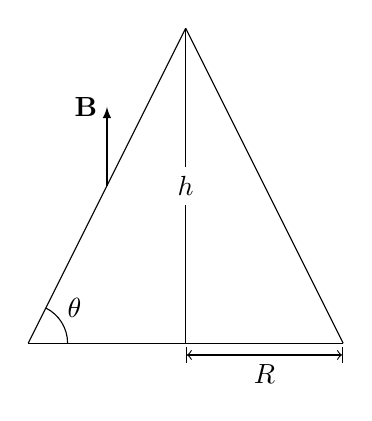
\begin{tikzpicture}
						\draw (-2, 0) -- (2, 0);
						\draw (-2, 0) -- (0, 4);
						\draw (2, 0) -- (0, 4);
						\draw (0, 0) -- (0, 4) node[midway, fill = white] {$h$};
						\draw[|<->|] (0, -0.15) -- (2, -0.15) node[midway, below] {$R$};
						\draw [-latex] (-1, 2) -- (-1, 3) node[left] {$\mathbf{B}$};
						\draw (-1.5, 0) arc (0:63.4349:0.5);
						\node at (-1.2, 0.2) [anchor = south east] {$\theta$};
					\end{tikzpicture}
				\end{figure}
				So $\cos\theta=\frac{R}{\sqrt{R^2+h^2}}$.
				\[
					\iint_{S_2}\mathbf{B}\cdot\hat{\mathbf{n}}\,dS=B\cos\theta\cdot A=\pi R^2B
				\]
				The two integrals add up to be zero.
			\end{item}
		\end{enumerate}
	}
\end{homeworkProblem}

%----------------------------------------------------------------------------------------
%	PROBLEM 5
%----------------------------------------------------------------------------------------

\begin{homeworkProblem}
	(2.31) Finding the potential... (problem omitted)
	% Question

	\problemAnswer{
		Through waypoint $(x_1,0,0)$
		\[
			\int_{(0,0,0)}^{(x_1,0,0)}6xy\,dx=0
		\]
		\[
			\int_{(x_1,0,0)}^{(x_1,y_1,0)}(3x^2-3y^2)\,dy=3{x_1}^2y_1-{y_1}^3
		\]
		Through waypoint $(0,y_1,0)$
		\[
			\int_{(0,0,0)}^{(0,y_1,0)}(3x^2-3y^2)\,dy=-{y_1}^3
		\]
		\[
			\int_{(0,y_1,0)}^{(x_1,y_1,0)}6xy\,dx=3{x_1}^2y_1
		\]
		So the sums are the same! Now $\phi(x,y,z)=3x^2y-y^3$.
		\[
			\nabla\phi(x,y,z)=(6xy,3x^2-3y^2,0)
		\]
		Components are of the exact same form.
	}
\end{homeworkProblem}

%----------------------------------------------------------------------------------------
%	PROBLEM 6
%----------------------------------------------------------------------------------------

\begin{homeworkProblem}
	(2.43) Potential from a rod... (problem omitted)
	% Question

	\problemAnswer{
		For the point $(0,0,2d)$,
		\[
			\phi(0,0,2d)=\int\frac{\rho(x',y',z')\,dx'\,dy'\,dz'}{4\pi\epsilon_0r}=\int_{-d}^d\frac{\lambda\,dz}{4\pi\epsilon_0(2d-z)}=\frac{\lambda\ln3}{4\pi\epsilon_0}
		\]
		For the point $(x,0,0)$,
		\[
			\phi(x,0,0)=\int_{-d}^d\frac{\lambda\,dz}{4\pi\epsilon_0\sqrt{x^2+z^2}}=\frac{\lambda}{2\pi\epsilon_0}\ln\frac{d+\sqrt{x^2+d^2}}{x}
		\]
		So
		\[
			\ln3=2\ln\frac{d+\sqrt{x^2+d^2}}{x}\Rightarrow x=\sqrt{3}d
		\]
	}
\end{homeworkProblem}

%----------------------------------------------------------------------------------------
%	PROBLEM 7
%----------------------------------------------------------------------------------------

\begin{homeworkProblem}
	(2.61) Dipole field on the axes... (problem omitted)
	% Question

	\problemAnswer{
		On $z$ axis,
		\[
			E(r)=\left(\frac{1}{4\pi\epsilon_0}\frac{q}{(r-l/2)^2}-\frac{1}{4\pi\epsilon_0}\frac{q}{(r+l/2)^2}\right)\hat{\mathbf{z}}=\frac{q}{4\pi\epsilon_0r^2}\left(\frac{1}{(1-l/2r)^2}-\frac{1}{(1+l/2r)^2}\right)\hat{\mathbf{z}}
		\]
		Using the approximation $1/(1\pm\epsilon)\approx1\mp\epsilon$ this equals
		\[
			\frac{q}{4\pi\epsilon_0r^2}\left((1+l/2r)^2-(1-l/2r)^2\right)\hat{\mathbf{z}}=\frac{ql}{2\pi\epsilon_0r^3}\hat{\mathbf{z}}
		\]
		Exactly the same with Equation 2.36 in the case that $\theta=0$.

		On $x$ axis, $r=\sqrt{x^2+z^2}$ where $z=l/2$. $\sin\theta=\frac{z}{\sqrt{r^2+z^2}}=l/2r$. From $q$
		\[
			E=\frac{1}{4\pi\epsilon_0}\frac{q}{r^2}\left(\cos\theta\hat{\mathbf{x}}-\sin\theta\hat{\mathbf{z}}\right)
		\]
		from $-q$
		\[
			E=\frac{1}{4\pi\epsilon_0}\frac{-q}{r^2}\left(\cos\theta\hat{\mathbf{x}}+\sin\theta\hat{\mathbf{z}}\right)
		\]
		So add these two together,
		\[
			E=-\frac{1}{2\pi\epsilon_0}\frac{q}{r^2}\sin\theta\hat{\mathbf{z}}=-\frac{ql}{4\pi\epsilon_0r^3}\hat{\mathbf{z}}
		\]
		Exactly the same with Equation 2.36 in the case that $\theta=\pi/2$.
	}
\end{homeworkProblem}

%----------------------------------------------------------------------------------------
%	PROBLEM 8
%----------------------------------------------------------------------------------------

\begin{homeworkProblem}
	(3.75) Average of six points

	Let $\phi(x,y,z)$ be any function that can be expanded in a power series around a point $(x_0,y_0,z_0)$. Write a Taylor series expansion for the value of $\phi$ at each of the six points $(x_0+\delta,y_0,z_0)$, $(x_0-\delta,y_0,z_0)$, $(x_0,y_0+\delta,z_0)$, $(x_0,y_0-\delta,z_0)$, $(x_0,y_0,z_0+\delta)$, $(x_0,y_0,z_0-\delta)$, which symmetrically surround the point $(x_0,y_0,z_0)$ at a distance $\delta$. Show that, if $\phi$ satisfies Laplace's equation, the average of these six values is equal to $(x_0,y_0,z_0)$ through terms of the third order in $\delta$.
	% Question

	\problemAnswer{
		A Taylor expansion is
		\[
			f(x)=f(a)+{\frac{f'(a)}{1!}}(x-a)+{\frac{f''(a)}{2!}}(x-a)^{2}+{\frac{f'''(a)}{3!}}(x-a)^{3}+\cdots
		\]
		Laplace's equation is $\nabla^2\phi=0$.

		To take total derivative on $\phi(x,y,z)$ would complicate things. So for the points $(x_0+\delta,y_0, z_0)$ and $(x_0-\delta,y_0,z_0)$, the expansion could be taken on partial derivative respect to $x$.
		\[
			\phi(x,y,z)=\phi(x_0,y_0,z_0)+\frac{\partial\phi(x_0,y_0,z_0)}{\partial x}(x-x_0)+\frac{1}{2}\frac{\partial^2\phi(x_0,y_0,z_0)}{\partial x^2}(x-x_0)^{2}+\frac{1}{6}\frac{\partial^3\phi(x_0,y_0,z_0)}{\partial x^3}(x-x_0)^{3}+\cdots
		\]
		So
		\[
			\frac{1}{2}(\phi(x_0+\delta,y_0,z_0)+\phi(x_0-\delta,y_0,z_0))=\phi(x_0,y_0,z_0)+\frac{1}{2}\frac{\partial^2\phi(x_0,y_0,z_0)}{\partial x^2}\delta^2+\frac{1}{24}\frac{\partial^4\phi(x_0,y_0,z_0)}{\partial x^4}\delta^4+\cdots
		\]
		And follow the exact same steps, the average on $y$ and $z$ directions could be derived. The average of all six points is then
		\begin{align*}
			&\frac{1}{6}\left(\phi(x_0+\delta,y_0,z_0)+\phi(x_0-\delta,y_0,z_0)+\cdots+\phi(x_0,y_0,z_0-\delta)\right) \\
			&=\phi(x_0,y_0,z_0)+\frac{1}{3}\left(\frac{1}{2}\left(\frac{\partial^2\phi}{\partial x^2}+\frac{\partial^2\phi}{\partial y^2}+\frac{\partial^2\phi}{\partial z^2}\right)\delta^2+\frac{1}{24}\left(\frac{\partial^4\phi}{\partial x^4}+\frac{\partial^4\phi}{\partial y^4}+\frac{\partial^4\phi}{\partial z^4}\right)\delta^4+\cdots\right) \\
			&=\phi(x_0,y_0,z_0)+\frac{1}{3}\left(\frac{1}{2}\nabla^2\phi\delta^2+\frac{1}{24}\nabla^4\phi\delta^4+\cdots\right)=\phi(x_0,y_0,z_0)
		\end{align*}
		Thus the average of these six values is equal to $(x_0,y_0,z_0)$.
	}
\end{homeworkProblem}

%----------------------------------------------------------------------------------------
%	PROBLEM 9
%----------------------------------------------------------------------------------------

\begin{homeworkProblem}
	(3.76) The relaxation method... (problem omitted)
	% Question

	\problemAnswer{
		This problem is straightforward, once the idea is understood. The numbers are supposed to converge to a certain value that we want to know with each iteration of the specified operations. However the process of finding the average of sum of the neighbors for each point seems to be tedious. To reduce the labor, a Java program is written to do the calculation.
		\begin{multicols}{2}
			\begin{table}[H]
				\centering
				\begin{tabular}{c c c c}
					0.000  &  25.000  &  50.000  &  100.000   \\
					0.000  &  25.000  &  50.000  &  100.000   \\
					0.000  &  25.000  &  50.000  &  100.000   \\
					0.000  &  25.000  &  50.000  &  50.000    \\
					0.000  &  25.000  &  25.000  &  25.000    \\
					0.000  &  0.000   &  0.000   &  0.000     \\
				\end{tabular}
				\caption{Initial conditions}
			\end{table}
			\begin{table}[H]
				\centering
				\begin{tabular}{c c c c}
					0.000  &  25.000  &  56.250  &  100.000   \\
					0.000  &  25.000  &  56.250  &  100.000   \\
					0.000  &  25.000  &  56.250  &  100.000   \\
					0.000  &  25.000  &  37.500  &  56.250    \\
					0.000  &  12.500  &  25.000  &  25.000    \\
					0.000  &  0.000   &  0.000   &  0.000     \\
				\end{tabular}
				\caption{Iteration 1}
			\end{table}
			\begin{table}[H]
				\centering
				\begin{tabular}{c c c c}
					0.000  &  26.563  &  59.375  &  100.000   \\
					0.000  &  26.563  &  59.375  &  100.000   \\
					0.000  &  26.563  &  54.688  &  100.000   \\
					0.000  &  18.750  &  40.625  &  54.688    \\
					0.000  &  12.500  &  18.750  &  26.563    \\
					0.000  &  0.000   &  0.000   &  0.000     \\
				\end{tabular}
				\caption{Iteration 2}
			\end{table}
			\begin{table}[H]
				\centering
				\begin{tabular}{c c c c}
					0.000  &  28.125  &  60.156  &  100.000   \\
					0.000  &  28.125  &  60.156  &  100.000   \\
					0.000  &  25.000  &  56.641  &  100.000   \\
					0.000  &  19.922  &  36.719  &  56.641    \\
					0.000  &  9.375   &  19.922  &  25.000    \\
					0.000  &  0.000   &  0.000   &  0.000     \\
				\end{tabular}
				\caption{Iteration 3}
			\end{table}
			\end{multicols}
			\begin{multicols}{2}
			\begin{table}[H]
				\centering
				\begin{tabular}{c c c c}
					0.000  &  28.320  &  61.230  &  100.000   \\
					0.000  &  28.320  &  61.230  &  100.000   \\
					0.000  &  26.172  &  55.469  &  100.000   \\
					0.000  &  17.773  &  38.281  &  55.469    \\
					0.000  &  9.961   &  17.773  &  26.172    \\
					0.000  &  0.000   &  0.000   &  0.000     \\
				\end{tabular}
				\caption{Iteration 4}
			\end{table}
			\begin{table}[H]
				\centering
				\begin{tabular}{c c c c}
					0.000  &  28.931  &  61.255  &  100.000   \\
					0.000  &  28.931  &  61.255  &  100.000   \\
					0.000  &  25.391  &  56.421  &  100.000   \\
					0.000  &  18.604  &  36.621  &  56.421    \\
					0.000  &  8.887   &  18.604  &  25.391    \\
					0.000  &  0.000   &  0.000   &  0.000     \\
				\end{tabular}
				\caption{Iteration 5}
			\end{table}
			\begin{table}[H]
				\centering
				\begin{tabular}{c c c c}
					0.000  &  28.894  &  61.652  &  100.000   \\
					0.000  &  28.894  &  61.652  &  100.000   \\
					0.000  &  25.989  &  55.817  &  100.000   \\
					0.000  &  17.725  &  37.512  &  55.817    \\
					0.000  &  9.302   &  17.725  &  25.989    \\
					0.000  &  0.000   &  0.000   &  0.000     \\
				\end{tabular}
				\caption{Iteration 6}
			\end{table}
		\end{multicols}
		As shown above, after six iterations, the difference of each point between the current state and previous state is less than 1 unit. The sketch is shown below.
		\begin{figure}[H]
			\centering
			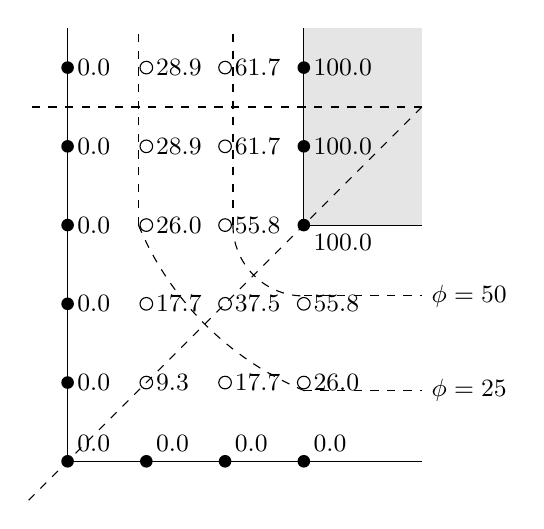
\begin{tikzpicture}[font = \small]
				\fill[gray!20] (-3/2, 1) rectangle (0, -3/2);
				\draw (-1.5, 1) -- (-1.5, -1.5);
				\draw (-1.5, -1.5) -- (0, -1.5);
				\draw (-9/2, 1) -- (-9/2, -9/2);
				\draw (-9/2, -9/2) -- (0, -9/2);
				\draw[dashed] (0, 0) -- (-5, 0);
				\draw[dashed] (0, 0) -- (-5, -5);
				% 50
				\draw[dashed] (-2.4, -1.5) arc (180:270:0.9);
				\draw[dashed] (-2.4, -1.5) -- (-2.4, 1);
				\draw[dashed] (-1.5, -2.4) -- (0, -2.4) node[right] {$\phi=50$};
				% 25
				\draw[dashed] (-3.6, -1.5) arc (202.62:248:3.9);
				\draw[dashed] (-3.6, -1.5) -- (-3.6, 1);
				\draw[dashed] (-1.5, -3.6) -- (0, -3.6) node[right] {$\phi=25$};
				% 1
				\fill (-3/2, 1/2) circle[radius = 0.08] node[right] {100.0};
				\fill (-3/2, -1/2) circle[radius = 0.08] node[right] {100.0};
				\fill (-3/2, -3/2) circle[radius = 0.08] node[anchor = north west] {100.0};
				\draw (-3/2, -5/2) circle[radius = 0.08] node[right] {55.8};
				\draw (-3/2, -7/2) circle[radius = 0.08] node[right] {26.0};
				% 2
				\draw (-5/2, 1/2) circle[radius = 0.08] node[right] {61.7};
				\draw (-5/2, -1/2) circle[radius = 0.08] node[right] {61.7};
				\draw (-5/2, -3/2) circle[radius = 0.08] node[right] {55.8};
				\draw (-5/2, -5/2) circle[radius = 0.08] node[right] {37.5};
				\draw (-5/2, -7/2) circle[radius = 0.08] node[right] {17.7};
				% 3
				\draw (-7/2, 1/2) circle[radius = 0.08] node[right] {28.9};
				\draw (-7/2, -1/2) circle[radius = 0.08] node[right] {28.9};
				\draw (-7/2, -3/2) circle[radius = 0.08] node[right] {26.0};
				\draw (-7/2, -5/2) circle[radius = 0.08] node[right] {17.7};
				\draw (-7/2, -7/2) circle[radius = 0.08] node[right] {9.3};
				\foreach \i in {1,-1,...,-7} {
					\fill (-9/2, \i/2) circle[radius = 0.08] node[right] {0.0};
				}
				\foreach \i in {-9,-7,-5,-3} {
					\fill (\i/2, -9/2) circle[radius = 0.08] node[anchor = south west] {0.0};
				}
			\end{tikzpicture}
		\end{figure}
	}
\end{homeworkProblem}

%----------------------------------------------------------------------------------------
%	PROBLEM 10
%----------------------------------------------------------------------------------------

\begin{homeworkProblem}
	We considered a potential $\phi(x,y)=x^2-y^2$. This scalar function satisfies LaPlace's equation so Theorem 2.1 in P\&M applies. For a scalar function that satisfies LaPlace's equation, the average value of the function on the surface of any sphere is equal to the value of the function at the center of the sphere.

	This is a 2D problem so a circle surrounding the point $(x_0, y_0)$ serves as the sphere. Calculate the average value of φ on a circle of radius $r$ centered at $(x_0, y_0)$ by computing the value of the line integral $\oint\phi(x,y)\,dl$ around the circle and then dividing the value of the integral by the arc length $2πr$. (This integral is easier to do after converting to circular coordinates.)
	% Question

	\problemAnswer{
		Theorem 2.1 If $\phi(x,y,z)$ satisfies Laplace's equation, then the average value of $\phi$ over the surface of any sphere (not necessarily a small sphere) is equal to the value of $\phi$ at the center of the sphere.

		Convert the problem into polar coordinates. In other words, $x=r\cos\theta$, and $y=\sin\theta$. So
		\[
			\oint\phi(x,y)\,dl=r^2\oint(\cos^2\theta-\sin^2\theta)\,dl=r^2\int_0^{2\pi}\cos2\theta\,d\theta=0
		\]
		Which agrees with $\phi(0,0)=0$. The theorem is verified in this case.
	}
\end{homeworkProblem}

%----------------------------------------------------------------------------------------

\end{document}
